\documentclass[10pt]{article}
\usepackage{pdfpages}

\usepackage{eucommon}
\usepackage{hyperref}
\geometry{a4paper, portrait, margin=20mm}

\usepackage{wrapfig}
\usepackage{graphicx}
\graphicspath{ {./images/} }

\setlength\parskip{0.5\baselineskip}

\newstaticframe[1]{\paperwidth}{\paperheight}{-20mm}{-20mm}[backgroundOverview]

\begin{document}
\thispagestyle{empty}
\ifrenderbw
\else
  \begin{staticcontents*}{backgroundOverview}
    \adjustbox{trim=0 0 {0.6666\width} 0,clip}{\includegraphics[height=\paperheight]{images/background.png}}
  \end{staticcontents*}
\fi

\sectionbg{EU:tPoP Reference Sheet}

This is a reference sheet for those who want something more verbose than official Player Aid,
but less verbose than Rules.
It includes most of the rules and presents them as bullet points.
It does not include setup rules and some things that can be understood more intuitively (e.g. some definitions on pages 3-5).


The content is fitted on 12 A4-size pages which are grouped in 3:
3 pages for Sequence of Play, 3 pages for Actions other than Military Actions,
3 pages for Military Actions, and finally, 3 pages containing Other Rules.
In some places, words are abbreviated and articles dropped to save space.
Therefore, all statements are not grammatically correct sentences, but hopefully they are still easily understandable.


\begin{wrapfigure}[10]{r}[0mm]{85mm}
  \centering
  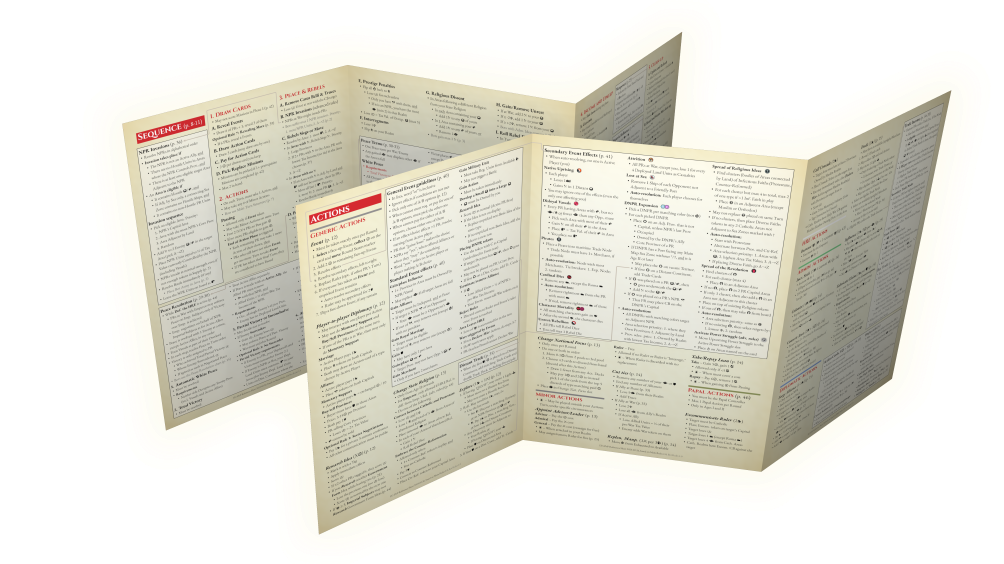
\includegraphics[width=85mm]{trifold.png}
\end{wrapfigure}

The pages are meant to be joined to form two 3\texttimes A4-size foldable sheets so that
one of them would contain Sequence of Play and Other Rules on opposite sides,
and the other one would have all the Actions (see image on the right).
To achieve this using a regular office printer, print (2-sided) one of the "trifold" files listed below,
and join the pages in groups of three as shown in the image.
If you do not want to bind them in such manner, then use one of the "single pages" files instead.

\subsection*{Available files}

Latest version of PDFs and \LaTeX\xspace sources can be found at \href{https://github.com/raunc/eutpop-ref-sheet}{https://github.com/raunc/eutpop-ref-sheet}.

\subsubsection*{PDF files}
\begin{description}[itemsep=0pt, parsep=0pt, leftmargin=0pt, labelsep=0pt]
  \item[\href{https://raw.githubusercontent.com/raunc/eutpop-ref-sheet/main/pdf/eutpop\_ref\_sheet.pdf}{eutpop\_ref\_sheet.pdf} \normal{(this file)}]
  ~--~All pages joined in groups of 3
  \item[\href{https://raw.githubusercontent.com/raunc/eutpop-ref-sheet/main/pdf/eutpop\_ref\_sheet\_single\_pages.pdf}{eutpop\_ref\_sheet\_single\_pages.pdf}]
  ~--~Single pages in logical order
  \item[\href{https://raw.githubusercontent.com/raunc/eutpop-ref-sheet/main/pdf/eutpop\_ref\_sheet\_single\_pages\_bw.pdf}{eutpop\_ref\_sheet\_single\_pages\_bw.pdf}]
  ~--~Single pages in logical order, no colored background and text
  \item[\href{https://raw.githubusercontent.com/raunc/eutpop-ref-sheet/main/pdf/eutpop\_ref\_sheet\_single\_pages\_flattened.pdf}{eutpop\_ref\_sheet\_single\_pages\_flattened.pdf}]
  ~--~Single pages in logical order, no transparent objects or vector graphics, 720dpi. More reliable for printing, but larger file size and text is not searchable
  \item[\href{https://raw.githubusercontent.com/raunc/eutpop-ref-sheet/main/pdf/eutpop\_ref\_sheet\_trifold.pdf}{eutpop\_ref\_sheet\_trifold.pdf}]
  ~--~Single pages reordered for binding as a trifold (see image and description above)
  \item[\href{https://raw.githubusercontent.com/raunc/eutpop-ref-sheet/main/pdf/eutpop\_ref\_sheet\_trifold\_bw.pdf}{eutpop\_ref\_sheet\_trifold\_bw.pdf}]
  ~--~Single pages reordered for binding as a trifold (see image and description above), no colored background and text
  \item[\href{https://raw.githubusercontent.com/raunc/eutpop-ref-sheet/main/pdf/eutpop\_ref\_sheet\_trifold\_flattened.pdf}{eutpop\_ref\_sheet\_trifold\_flattened.pdf}]
  ~--~Single pages reordered for binding as a trifold (see image and description above), no transparent objects or vector graphics, 720dpi. More reliable for printing, but larger file size and text is not searchable
\end{description}

Note that these links point to the latest version of the files, which might differ from this file.

\subsection*{Formatting}

Main Rules are written in black (or {\color{redTextColor}red} in some cases). These apply to both human players and bots,
unless inapplicable to bots (e.g bots do not deal with \ducats).
\botrule{Bot Rules are written in dark gray (or {\color{redBotTextColor}light red} in some cases). These are relevant only when bots are in play.}
References to specific pages (e.g. \dprime(p.~2)\dprime) also follow the same colors.
They are written in black when they refer to Main Rules and \botrule{in dark gray}
when they refer to Bot Rules.

\subsection*{Note about rulebook versioning}

Page footers say that this work is based on Rules 1.0, which is the latest version published online at the time of writing. However, printed rulebook (the one that comes with the game) is not identical to the online version. The only significant difference known to the authors of this reference sheet is the definition of Conquest CB on page 22 of Rules. This change has been made here too, but the version still points to 1.0 because the printed rulebook has no version number on it.

\includepdf[pages=-,fitpaper]{../build/joined\filenamesuffix.pdf}

\end{document}
